\section{AFND Números binarios con terminación '01'}
	\subsection{Descripción del problema}
	Desarrollar un autómata finito no determinista, que acepte todas y sólo las cadenas formadas por ceros y unos que terminan en 01. Asimismo, imprimir la tabla de transiciones (historia) y que la entrada de cadenas sea de forma manual o automática, la cadena automática debe de tener una longitud $n \mid 1  \leq n \leq 1000$. Y que contenga la opción de mostrar el siguiente diagrama.
	\begin{figure}[ht]
		\begin{center}
			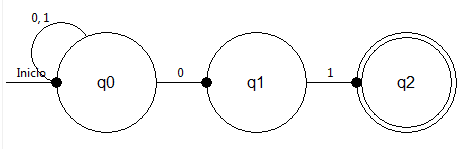
\includegraphics[width=12cm, height=4cm]{img/cero-uno.png}
			\caption{Diagrama de transiciones del autómata. \cite{LIBRO}}
			\label{fig:diagrama4}
		\end{center}
	\end{figure}
	
	\subsection{Código}
	El código fue realizado en Python 3.5.
	\subsection{Pruebas}
	Pruebas de las opciones del menú.
	{\large Modo automático.}
	{\large Modo manual.}
	{\large Diagrama.}